\chapter{Introducción a la Teoría de Grupos}


\section{Introducción histórica}
Hoy en día, la Teoría de Grupos es una rama de las matemáticas plenamente consolidada. Sin embargo, esta teoría surge por la abtracción de muchas ideas que se han ido desarrollando paralelamente durante el transcurso de los siglos.

A finales del siglo XVIII, Lagrange (1736, 1813) estudió diferentes métodos para la resolución de ecuaciones polinómicas de grado tres y cuatro. Más tarde, Ruffini (1765-1822) afirmó que a partir de la ecuación quinta, las ecuaciones polinómicas no son resolubles por radicales. Esta demostración no se realizó hasta 1824 por Abel (1802,1829) y hoy en día se conoce como \textit{Teorema de Abel-Ruffini}.  En términos modernos esto quiere decir que $A_n$ es simple y  $S_n$ no es resoluble para $n\geq 5$. Otra  contribución destacable de Ruffini fue el estudio del grupo de Permutaciones, que más adelante usó Cauchy (1789,1857) para desarrollarla y dar lugar a la Teoría de Grupos de Permutaciones. 

Todos estos estudios fueron precursores y contribuyeron en gran medida al trabajo realizado por Galois (1811-1832), un joven francés que revolucionó el mundo de las Matemáticas y, en particular, el concepto de \textit{<<Grupo>>}. A la temprana edad de 17 años, Galois escribió uno de sus primeros artículos, que se basaba en dar criterios sobre la resolubilidad de la ecuación polinómica por radicales.  Además, escribió otros artículos dirigidos a la Academia de Ciencias Francesa, siendo todos rechazados por ser ``incomprensibles y carecer de rigor''. Entre sus estudios, agrupados en lo que se conoce como la \textit{Teoría de Galois} o \textit{Teoría de Grupos} y recogidas en \textit{Oeuvres mathématiques d'Évariste Galois}, se destaca el grupo de Permutaciones o el grupo de Galois de un polinomio.


En 1851, Betti (1823,1892) relacionó la Teoría de Permutaciones y Teoría de Ecuaciones. Además, consigue demostrar que el grupo de Galois asociado a una ecuación es, en el sentido moderno, un grupo de permutaciones. A raíz de su trabajo, en 1870, Jordan (1838,1922) define el concepto de isomorfismo entre ellos. Además, prueba lo que hoy se conoce como el \textit{Teorema de Jordan-Hölder}, que garantiza la existencia y unicidad, salvo isomorfismos, de series de composición para estos grupos.


Debemos destacar al matemático Walter von Dyck, (1856, 1934) quien, con la ayuda de Klein (1849,1925) dio una construcción de grupos libres y una definición de grupo dado por generadores y relatores, agrupados bajo el nombre de presentación de grupo.

En 1854, Cayley (1821,1895) define el concepto de grupo abstracto mediante una tabla de multiplicación que refleja los elementos. Posteriormente, publica varios artículos en los que demuestra que los cuaternios y las matrices forman un grupo. Además, demuestra el teorema que hoy en día lleva su nombre, el \textit{Teorema de Cayley}, que sostiene que todo grupo puede describirse en términos de permutaciones.

A partir de este momento, fueron muchos los matemáticos quienes contribuyeron a construir la Teoría de Grupos que hoy en día conocemos.  Podríamos destacar las investigaciones realizadas sobre grupos y subgrupos de orden primo.  Los estudios de Cayley motivaron a Hölder (1859,1937), y en 1893 comenzó a investigar grupos cuyo orden es producto de números primos. Cabe destacar también a Sylow (1832,1918), quien enunció y demostró los teoremas que hoy en día llevan su nombre, y que nos proporcionan información sobre el número de subgrupos de orden fijo contenidos en un grupo finito dado.



%Por último, cabe destacar a \textit{Sylow, (1832,1918)} junto con los teoremas que hoy en día llevan su nombre, los \textit{Teoremas de Sylow}.
%Estos, relacionan un grupo con los p-subgrupos de Sylow y nos proporcionarán las principales herramientas para poder clasificar los grupos no abelianos.

\section{Objetivos}
El principal objetivo del presente trabajo es el de desarrollar el trabajo realizado por Dyck, estudiando la construcción de grupos libres y principales problemas que surgen a raíz de éstos. Esta construcción  permitirá definir grupos mediante un conjunto de generadores y relatores, que se usará en \ref{semidirect1} (junto a las acciones de grupo) para introducir el producto semidirecto de grupos. Además, se estudiará principalmente la clasificación de grupos cuyo orden es producto de números primos, al igual que hizo Hölder.


En relación con la parte informática, se implementarán los principales grupos y se completarán y añadirán a la librería mencionada anteriormente nuevos métodos relacionados con la parte matemática.
Uno de los problemas que surgen al dar un grupo mediante una presentación, es determinar si dos palabras definen el mismo elemento, o equivalentemente, cuándo una palabra define el elemento neutro. Este problema se conoce como Problema de Palabras, y para resolverlo se llevará a cabo una descripción e implementación del \textit{Algoritmo de Todd Coxeter}, lo que  permitirá definir grupos dados mediante una presentación. Asimismo, se deberán usar los métodos de la librería para identificar el grupo finitamente presentado con uno conocido.




La principales fuentes de bibliografía consultadas para la parte matemática han sido: ~\cite{abstractrojo}, ~\cite{abstract}, ~\cite{milneGT}, ~\cite{free} y ~\cite{Barrera}, y para informática: ~\cite{green}, ~\cite{tool}, ~\cite{kmill} y ~\cite{Pedrito}.



\newpage


\section{Conceptos previos}

A modo introductorio, definiremos en esta primera sección el concepto de grupo y algunas propiedades elementales sobre éstos, que nos facilitarán el entendimiento de los principales teoremas de la Teoría de Grupos utilizados en el desarrollo del trabajo. Seguiremos en \ref{acciones} explicando las acciones de grupo, y en \ref{sylows} enunciando los \textit{Teoremas de Sylow}, que nos serán de mucha utilidad en las secciones posteriores.
No se incluyen las demostraciones por ser un material clásico presente en cualquier curso sobre Teoría de Grupos.  El lector puede consultar  ~\cite{bueso} o ~\cite{milneGT} para una descripción más detallada.

\begin{definition} \label{defgrupo}
Un grupo es una cuaterna $(G,\bigcdot,^{-1},1)$, donde $G$ es un conjunto no vacío, $\bigcdot:G\times G\rightarrow G$ es una operación binaria, $^{-1}:G\rightarrow G$ es una operación unaria y $1\in G$ es un elemento. Tales que se cumplen las siguientes propiedades:
\end{definition}

\begin{enumerate}
\item \textit{Asociatividad}:
	 $x\bigcdot(y\bigcdot z) = (x\bigcdot y)\bigcdot z$, para todo $x,y,z \in G$.
	 
\item \textit{Existencia de elemento neutro}:  $x\bigcdot 1 = 1\bigcdot x$,  para todo $x\in G$.

\item \textit{Existencia de elemento simétrico}: $x\bigcdot x^{-1} = x^{-1}\bigcdot x =1$,  para todo $x\in G$.
\end{enumerate}

Adicionalmente, si la operación binaria sobre $G$ cumple la propiedad conmutativa, esto es: $x\bigcdot y=y\bigcdot x$, para todo $x,y\in G$,  diremos que el grupo es \textit{abeliano} o \textit{conmutativo}.







\begin{definition}
	Sea $H$ un subconjunto no vacío de un grupo $G$. $H$ es un subgrupo de $G$  si verifica las siguientes propiedades:

\begin{enumerate}
	\item Si $x,y \in H$ , entonces $xy \in H$,
	\item Si $x \in H$ , entonces $x^{-1} \in H$.
\end{enumerate}
\end{definition}



\begin{definition}
Un grupo $G$ es finito si contiene un número finito de elementos. A este número lo denominaremos orden del grupo $G$ y se denotará por $|G|$.
\end{definition}


\begin{definition}
 El orden de un elemento $x\in G$, denotado por $|x|$, es el menor entero positivo $n$  que cumple $x^n = 1$. Si no existe tal $n$, se dice que $x$ tiene un orden infinito. 
\end{definition}







Mostramos diferentes grupos que se usarán con posterioridad:
\begin{Ejemplo} \label{ejemplosgr}
\hfill
\begin{itemize}
    \item $\mathbb{Z}_n$, $n\in \mathbb{N}$, el conjunto de las clases de equivalencia de los enteros $0,1,\ldots, n-1$ módulo $n$.
    
    \item Sea $X$ un conjunto no vacío. El conjunto de todas las aplicaciones biyectivas  de $X$ en sí mismo forman un grupo bajo la composición de funciones, que será denotado por $S_X$. Si $X$ es el conjunto finito $\{1,2,\ldots n\}$, entonces el grupo $S_X$ se denotará por $S_n$ y se llamará grupo Simétrico.
    
    \item El conjunto de las permutaciones pares del conjunto $\{1,2, \ldots,n\}$ es un subgrupo de $S_n$ que se conoce como grupo Alternado, denotado por $A_n$.

    \item Sea $P$ un polígono regular de $n$ lados. El grupo Diédrico $D_n$ vendrá dado por las isometrías que preservan dicho polígono: las $n$ rotaciones y $n$ reflexiones. 
    \[
    D_n =\{ \underbrace{1,\varphi, \varphi^2,...,\varphi^{n-1}}_{\text{$n$ rotaciones}},
    \underbrace{\sigma, \sigma\varphi,...,\sigma\varphi^{n-1}}_{\text{$n$ simetrías}}\} .
    \]
    
    %bajo las siguientes operaciones:
    %\[
   % \varphi_i \varphi_j = \varphi_{i+j} \qquad \varphi_i %\sigma_j = \sigma_{i+j} \qquad \sigma_i \varphi_j = %\sigma_{i-j} \qquad \sigma_i \sigma_j = \varphi_{i-j}
    %\]
    
    \item Sea $n$ un número natural. Consideremos el conjunto de los números complejos que cumplen $z^n=1$:
    \[
    \mathbb{C}_n = \{ z \in \mathbb{C}: z^n =1    \} .
    \]
    El conjunto $\mathbb{C}_n$ bajo la multiplicación usual de los números complejos se conoce como grupo de las raíces n-ésimas de la unidad, donde cada raíz compleja viene dada por:
    \[
    \zeta_k = e^{\frac{2\pi ki}{n}} = cos(\frac{2\pi k}{n}) + isen(\frac{2\pi k}{n}) \: \text{ con } k = 0,\ldots,n-1 .
    \]

    
    \item Los cuaternios son una extensión de los números reales, similar a los números complejos, donde se usan tres unidades imaginarias $i, j, k$ que verifican:
    \begin{align*}
    i^2 = j^2=k^2 = ijk = -1\: .
    \end{align*}
    
    El conjunto $\{\pm{1}, \pm{i}, \pm{j}, \pm{k} \}$ se denomina grupo de los Cuaternios y se denota por $Q_2$.



\end{itemize}
\end{Ejemplo}




El siguiente teorema será de gran importancia en la parte de informática ya que podremos representar los elementos de un grupo como permutaciones.
\begin{theorem}[Cayley] \label{cayley}
Todo grupo es isomorfo a un subgrupo de un grupo de Permutaciones.
\end{theorem}



\begin{theorem}
Sea $G$ un grupo y $x$ un elemento de $G$. El subgrupo cíclico generado por $x$ se define como $\langle x \rangle = \{x^n, \: n \in \mathbb{Z}\}$. Cuando todo el grupo $G$ es generado por alguno de sus elementos entonces $G$ es cíclico y se denotará $G= \langle x \rangle$.
\end{theorem}

















\begin{definition} \label{clases}
    Sea $H$ un subgrupo de $G$. Se define la clase lateral a izquierda de un elemento $x \in G$ respecto de $H$ como:
    \[
        xH = \{ xh;\: h \in H \}.
    \]
    De igual modo, la clase lateral a derecha de $x$ respecto a $H$ viene dada por:
    \[
        Hx = \{ hx; \: h \in H\}.
    \]
    
    El número de clases laterales izquierda coincide con el número de clases laterales derechas, se denomina índice de $H$ en $G$ y se denota por $[G:H]$.
    

\end{definition}


\newpage
A continuación enunciamos el \textit{Teorema de Lagrange}, uno de los teoremas más importantes de la Teoría de Grupos ya que tiene implicaciones muy importantes en el estudio de grupos finitos.

\begin{theorem}[Lagrange] \label{Lagrange}
Sea $H$ un subgrupo de un grupo finito $G$. Entonces, el orden de $H$ divide al orden de $G$. En particular, se cumple:
\[
    |G| = [G:H]\cdot|H|\:.
\]
\end{theorem}






\begin{definition}
	Un subgrupo $H$ de un grupo $G$ se dice que es un subgrupo normal de $G$ y se denotará $H \unlhd G$ si $xH=Hx$, para todo $x \in G$. 
\end{definition} 


El siguiente teorema servirá para demostrar la normalidad de un subgrupo.
\begin{theorem}
Un subgrupo $H$ de un grupo $G$ es normal si, y sólo si, $xHx^{-1} \subseteq H$, para todo $x \in G$.
\end{theorem}


Los subgrupos normales tienen especial importancia. Cuando un subgrupo $H$ es normal en $G$, entonces el conjunto de las clases laterales a izquierda y a derecha coinciden; de hecho, forman un grupo llamado Grupo Cociente, que será denotado por $G/H$. Enunciamos el siguiente teorema:

\begin{theorem}
Sea $H$ un subgrupo normal de un grupo $G$. El conjunto $G/H = \{ Hx, \: x \in G\}$ es un grupo con la operación $(Hx)(Hy)=Hxy$.
\end{theorem}





Terminamos este primer capítulo introductorio recordando el concepto de homomorfismo de grupos.

\begin{definition}
Sean $G$ y $G'$ dos grupos. Un homomorfismo de grupos de $G$ en $G'$ es una aplicación $\varphi \colon G \to G'$ que satisface $\varphi(x,y)=\varphi(x)\varphi(y)$, para todo $x, y \in G$.


%\begin{remark}
 %Un \textit{monomorfismo} es un morfismo inyectivo. Si dicho morfismo es sobreyectivo, se llama \textit{epimorfismo} y, si es biyectivo, \textit{isomorfismo}.
%Un \textit{endomorfismo} es un morfismo de un grupo en sí mismo mientras que un \textit{automorfismo}  es un {isomorfismo endomorfo}.

%\end{remark}
\end{definition}

\begin{definition}
    Un isomorfismo es un homomorfismo de grupos biyectivo. Dos grupos $G$ y $G'$ serán isomorfos y se denotará por $G \cong G'$ si existe un isomorfismo entre ellos.
    Un isomorfismo de un grupo $G$ en sí mismo es llamado automorfismo de $G$ y se denota por Aut($G$) al conjunto de todos los automorfismo de $G$.
\end{definition}



\newpage
\subsection{Acciones de grupo} \label{acciones}

En primer lugar, se estudiará el caso de grupos actuando sobre conjuntos, idea que nos permitirá obtener más información sobre la estructura del grupo. Después veremos la teoría necesaria para hacer actuar a un grupo sobre otro.

\begin{definition} \label{prop}
    Sea $X$ un conjunto y $G$ un grupo. Una acción (izquierda) de $G$ sobre $X$ es una aplicación $G \times X \rightarrow X;  \; (g,x) \mapsto {}^{g}x$ que cumple las propiedades:
    \begin{enumerate}
        \item ${}^{1}x = x$, $\quad \forall x \in X$.\label{es1}
        \item ${}^{g}({}^{g'}x)={}^{g{g'}}x$,  $\quad \forall x \in X $, $\forall g, g' \in G$. \label{es2}
    \end{enumerate}
\end{definition}

En tal caso se dice que $G$ actúa sobre $X$, y que el conjunto $X$ es un $G$-conjunto.


De forma análoga, se pueden definir acciones a derechas:
\begin{align*}
 G \times X &\rightarrow X \\
 (g,x) &\mapsto x^g
\end{align*}
Estas nos serán de mucha utilidad más adelante en la Sección \ref{TC}, cuando se proceda a describir el \textit{Algoritmo de Todd Coxeter}.



%Esto lo he quitado, si se supone que es un recordatorio mejor ser breve y conciso que enrrollarme con ejemplos.
%Para ver como quedaría descomenta \iffalse de la siguiente línea y \fi de la línea 354
\iffalse
\begin{Ejemplo}
Sea $D_4$ el grupo de simetrías y rotaciones del cuadrado y $X=\{1,2,3,4\}$ el conjunto de sus vértices.

Si consideramos $D_4$ como el conjunto de las permutaciones:
\[
    \{ 1, (13),(24), (12)(34), (13)(24), (14)(23), (1234), (1432) \}
\]
se ve que $D_4$ actúa sobre $X$ de la siguiente forma:

\begin{center}
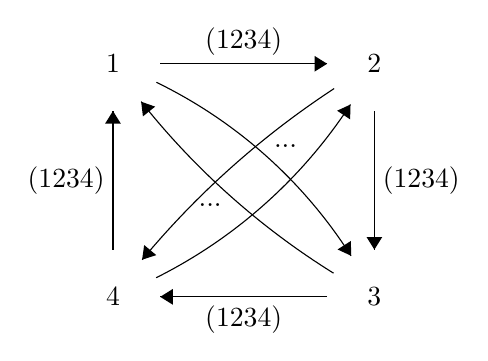
\begin{tikzpicture}[scale=0.2]
\tikzstyle{every node}+=[inner sep=0pt]
\draw (30.4,-33.8) node {$4$};
\draw (47,-33.8) node {$3$};
\draw (30.4,-19) node {$1$};
\draw (47,-19) node {$2$};
\draw [black] (44.405,-32.296) arc (-121.89264:-141.5456:47.94);
\fill [black] (32.19,-21.41) -- (32.3,-22.34) -- (33.08,-21.72);
\draw (36.57,-27.86) node [below] {$...$};
\draw [black] (47,-22) -- (47,-30.8);
\fill [black] (47,-30.8) -- (47.5,-30) -- (46.5,-30);
\draw (47.5,-26.4) node [right] {$(1234)$};
\draw [black] (32.255,-31.442) arc (140.24742:123.19082:55.069);
\fill [black] (32.25,-31.44) -- (33.15,-31.15) -- (32.38,-30.51);
\draw [black] (45.482,-21.586) arc (-33.13031:-63.43145:31.626);
\fill [black] (45.48,-21.59) -- (44.63,-21.98) -- (45.46,-22.53);
\draw [black] (33.158,-20.177) arc (64.06768:32.49408:30.427);
\fill [black] (45.52,-31.19) -- (45.51,-30.25) -- (44.66,-30.79);
\draw (41.36,-24.34) node [above] {$...$};
\draw [black] (44,-33.8) -- (33.4,-33.8);
\fill [black] (33.4,-33.8) -- (34.2,-34.3) -- (34.2,-33.3);
\draw (38.7,-34.3) node [below] {$(1234)$};
\draw [black] (30.4,-30.8) -- (30.4,-22);
\fill [black] (30.4,-22) -- (29.9,-22.8) -- (30.9,-22.8);
\draw (29.9,-26.4) node [left] {$(1234)$};
\draw [black] (33.4,-19) -- (44,-19);
\fill [black] (44,-19) -- (43.2,-18.5) -- (43.2,-19.5);
\draw (38.7,-18.5) node [above] {$(1234)$};
\end{tikzpicture}
\end{center}

La permutación trivial actúa sobre cada vértice enviándolo a sí mismo. Del mismo modo, $(1234)$ aplicada a un vértice se corresponde con un giro de $90^{\circ}$, llevando $1 \rightarrow 2 , \ldots , 4 \rightarrow 1$.
Un giro de $180^{\circ}$ es la composición de dos giros de $90^{\circ}$, es decir, $(1234)^2 = (13)(24)$, que al actuar sobre los distintos vértices envían $1\rightarrow 3, \; 2\rightarrow 4 \ldots $

\end{Ejemplo}
\fi
   
  
\begin{remark} \label{action}
%Se puede definir una acción dando un homomorfismo de $G$ sobre el grupo de biyecciones del conjunto $X$:
Sea $G$ un grupo y $X$ un conjunto no vacío. Dar una acción de $G$ sobre $X$ es equivalente a dar un homomorfismo de grupos $\phi \colon G \rightarrow S(X)$, el grupo de Permutaciones de X.
    \begin{align*}
        \phi \colon G &\longrightarrow S(X) \\
        g  &\longmapsto \phi(g) = \phi_g   \colon \; \; X\longrightarrow X \\
            & \hspace{3.5cm}   x \longmapsto \phi_g(x) = {}^gx
        %\varphi(k) &= \varphi_k
    \end{align*}
    
\end{remark}





%Como conjunto $X$ podemos tomar un grupo $H$ y así %restringirnos a las acciones de $G$ sobre $H$ que sean %compatibles con la estructura de grupo, es decir, acciones %que satisfagan:

%\begin{itemize}
%    \item $1_h=h $ , $\quad \forall h \in H$
%    \item $g(g'_h) = (gg')_h $ ,  $\quad \forall h \in H %$, $\forall g, g' \in G$
%\end{itemize}



%\begin{Ejemplo}
%El ejemplo más sencillo es la acción trivial:
%\begin{align*}
% %   {}^{g}x = x,  \quad \forall x\in X, \; %\forall g \in G .
%\end{align*}
%En este caso, la biyección $\phi_g$ lleva %cada elemento en sí mismo, es decir, es la %aplicación identidad del conjunto $X$.
%\end{Ejemplo}




\begin{definition}
    El \textit{núcleo} de una acción $\phi \colon G \times X \rightarrow X$ es el conjunto de los elementos de $G$ que actúan trivialmente sobre todo elemento del conjunto $X$:
    \[
        \operatorname{ker}(\phi)=\{ g \in G \; | \; {}^gx=x, \;\forall x \in X \} \: .
    \]
    Cuando $\phi$ es inyectivo, o equivalentemente el núcleo es trivial, decimos que la acción es \textit{fiel}. 
    
    En cambio, los elementos del conjunto $X$ sobre los que todos los elementos de $G$ actúan trivialmente son llamados \textit{puntos fijos}:
    \[
        \operatorname{Fix}(X)= \{ x \in X \; | \; {}^gx=x, \; \forall g \in G \} \: .
    \]
\end{definition}



%\begin{definition}
%Sea $G$ un grupo. El centro de $G$ es el subgrupo:
%	    \[
%	    Z(G) = \{ g \in G \;:\; gh=hg,  \forall h \in G  \}
%	    \]
%\end{definition}
%Es claro que el centro de un grupo es un subgrupo abeliano de $G$.





Ahora bien, en vez de considerar un conjunto $X$, podemos tomar otro grupo $H$, con $h,h'\in H$ y restringirnos a las acciones de $G$ sobre $H$ que sean compatibles con la estructura de grupo, es decir, acciones que satisfagan además:
\begin{enumerate}
    \item ${}^g1=1$ , \label{grupo1}
    \item ${}^g(hh') = {}^gh {}^gh'$ .\label{grupo2}
\end{enumerate}

Bajo estas condiciones, el grupo $H$ se denomina $G$-grupo.

Entonces, dar una acción de grupos de $G$ en $H$ equivale, por el Comentario \ref{action}, a dar un homomorfismo de grupos $G \rightarrow \operatorname{Aut}(H)$. Este concepto nos será de mucha utilidad en la sección \ref{semidirect1} ya que dará lugar a la construcción del producto semidirecto. Tenemos pues:
\begin{align*}
    G \times H &\rightarrow G \\
    (g,h) & \mapsto {}^gh
\end{align*}
o, equivalentemente el homomorfismo de grupos:
\begin{align*}
    \phi \colon G &\longrightarrow \operatorname{Aut}(H) \\
    g  &\longmapsto \phi(g) = \phi_g   \colon \; \; H\longrightarrow H \\
        & \hspace{3.5cm}   h \longmapsto \phi_g(h) = {}^gh
    %\varphi(k) &= \varphi_k
\end{align*}


%\begin{theorem}[Cayley] \label{cayley}
%Todo grupo finito de orden $n$ es isomorfo a un subgrupo de $S_n$.
%\end{theorem}






\begin{Ejemplo} \label{oth}
Sea $G$ un grupo actuando sobre sí mismo. La acción por \textit{traslación} se define como:
    \begin{align*}
         G\times G & \rightarrow G \\
        (g,x) & \mapsto {}^gx := gx
    \end{align*}
    
Claramente satisface la Definición \ref{prop} ya que:
\begin{enumerate}
    \item ${}^1x = 1x= x $,  
    \item ${}^{gg'}x = (gg')x = g(g'x) = {}^{g}({}^{g'}x) $.
\end{enumerate}  
Sin embargo, no es una acción de grupos ya que ${}^g1 = g\cdot1=g \not = 1$.
\end{Ejemplo}    



\begin{Ejemplo}
De igual modo que en \ref{oth}, la acción por \textit{conjugación} se define como:
    \begin{align*}
         G\times G & \rightarrow G \\
        (g,x) & \mapsto {}^gx := gxg^{-1}
    \end{align*}
    
Satisface la Definición \ref{prop} pues:
\begin{enumerate}
    \item ${}^1x = 1x1^{-1}=x $,
    \item  ${}^{gg'}x = (gg')x(gg')^{-1}=    g(g'xg'^{-1})g = {}^{g}({}^{g'}x) $.
\end{enumerate}  

Cumple \ref{grupo1} y \ref{grupo2} por lo que además es una acción de grupo.
\end{Ejemplo}  
    

%\begin{Ejemplo}
%    \texttt{Acción de las clases laterales}
%    Sea $G$ un grupo y $X=G/H$ el conjunto de clases laterales por la izquierda de un subgrupo $H$. La aplicación:
%    \begin{align*}
%        G \times X &\rightarrow X \\
%        (g, xH) &\mapsto g_{xH} := gxH 
%    \end{align*}
%    es una acción de $G$ sobre $X$. De hecho, cuando $H=1$ se tiene la acción por traslación anterior.
%    
%    \begin{proof}
%    \mbox{}\par
%    \begin{itemize}
%        \item $1_x = xH$
%        \item $(gg')_{xH} = gg'_{xH} = g(g'_{xH})$
%    \end{itemize}
%    \end{proof}
%\end{Ejemplo}  











\iffalse
\begin{definition}
	 Definimos la \textit{órbita} de un elemento $x \in X$ como:
    \begin{align*}
    	\mathcal{O_G}(x) = \{g_x \; | \; g\in G\} 
    \end{align*}
    Cuando la acción presenta una única órbita, decimos que es \textit{transitiva}.
\end{definition}



\begin{definition}
    Sea $H\leq G$, definimos el normalizador y centralizador de G en H como:
    \[
    N_G(H)= \{ x \in G; xH=Hx \} \leq G
    \]
    \[
    C_G(H) = \{ x \in G; xh=hx \hspace{0.2cm}\forall h \in H \} \trianglelefteq N_G(S)
    \]
\end{definition}




\begin{definition}
    Sea $G$ un grupo que actúa sobre un conjunto $X$.
    El \textit{centralizador} de un elemento $x\in X$ $C_G(x)$ viene dado por:
    \[
    C_G(x) = \{ g \in G : gx=xg \}
    \]
    mientras que el \textit{estabilizador}, $Stab_G(x)$, será un subgrupo de $G$ y vendrá dado por:
	\[
	    Stab_G(x) = \{ g \in G : g_x=x \} \leq G ;\quad x\in X
	\]
\end{definition}





\begin{theorem} \label{th1}
Sea G un grupo y X un G-conjunto. Si $x\in X$, entonces:
\[
    \text{\#}\mathcal{O_G}(x) = |\mathcal{O_G}(x)| = [G:Stab_G(x)]  
\]
y, por tanto:
\[
    |\mathcal{O_G}(x)| \big/ |G|
\]

\end{theorem}



\begin{definition}
Sea $G$ un grupo finito y $X$ un $G-$Conjunto que se puede expresar como:
\[
|X| = \sum_{x \in \gamma} {\mathcal{O}_G(x)} = Fix(X) + \sum_{x \in \gamma \setminus Fix(X)} {\mathcal{O}_G(x)}
\]


Considerando la acción por conjugación sobre $G$ definida en \ref{acc}:
\[
    |G| = |Z(G)| + |\mathcal{O}_G(x_1)| +...+ |\mathcal{O}_G(x_k)| \quad x_i \in \gamma \setminus Fix(X)
\]

Aplicando el Teorema \ref{th1} a la expresión anterior:
\[
    |G| = |Z(G)| + [ G:C_G(x_1)] +...+ [ G:C_G(x_k)] , \quad x_i \in \gamma \setminus Z(X)
\]
resultando en la \textbf{Fórmula de Clases}:
\[
    |G| = |Z(G)| + \sum_{x \in \gamma \setminus Z(X)}{ [ G:C_G(x)]} 
\]


\end{definition}

\begin{remark} 
Cuando en un grupo $G$ actúa la acción por conjugación, las órbitas de dicha acción se denominan \textbf{clases de conjugación}.
\end{remark}

\begin{Ejemplo}
Consideramos el grupo de permutaciones $S_3$. Las clases de conjugación son las siguientes:

\begin{equation*}
\begin{rcases}
  \{ 1\}  \\
   \{ (12),(23),(13) \} \\
   \{ (123),(232)\} 
\end{rcases}
\xRightarrow[\text{de clases}]{\text{Fórmula}}
1+3+2 = 6
\end{equation*}
\end{Ejemplo}

\fi 




\newpage 
\subsection{Teoremas de Sylow} \label{sylows}

%Solo de aquellos que tienen orden potencias de primos, además la mayor que divide al orden del grupo
Los \textit{Teoremas de Sylow} son nombrados en honor al matemático Ludwig Sylow y son de los teoremas más importantes en Teoría de Grupos ya que nos proporcionan información detallada  sobre los subgrupos de orden $p$, donde $p$ es un número primo. Entre sus aplicaciones destacamos su importancia en la clasificación de grupos no abelianos finitos.




%Sea $p$ un numero primo, se dice que $G$ es un \textit{p-grupo} si el orden de $G$ es una potencia de $p$. Si todo elemento $g\in G$ tiene orden una potencia de $p$, $G$ también será un $p$-grupo.


\begin{definition}
    Si $p$ es un primo, un grupo $G$ es un $p$-grupo si todo elemento tiene orden una potencia de $p$.
\end{definition}

El Teorema \ref{cauchy} nos permitirá probar que todo $p$-grupo finito tienen orden una potencia de $p$:

\begin{theorem}[Cauchy] \label{cauchy} Sea $G$ un grupo y $p$ un número primo tal que $p$ divide a $|G|$, entonces $G$ contiene un elemento de orden $p$.
\end{theorem}
\begin{remark}
Dado $G$ un grupo de orden $n$ y $p$ primo que divida al orden de $G$, el Teorema de Cauchy \eqref{cauchy} nos asegura la existencia de un subgrupo de orden $p$. Como consecuencia,  el orden de un $p-$grupo de orden finito es una potencia de $p$.
\end{remark}




%\begin{theorem}[Burnside] \label{burnside} Sea G un p-grupo finito no trivial, entonces $p \mid |Z(G)|$ y, por tanto, $Z(G) \not = 1$
%\end{theorem}







%Dado un número primo $p$, un \textit{p-subgrupo de Sylow} de un grupo $G$ es un grupo cuyo orden es una potencia de $p$ y que no está contenido en otro \textit{p-grupo}, es decir,  es maximal en $G$.
%Podemos enunciar ahora los Teoremas de Sylow, agrupados en el teorema \ref{sylow}.


Sea $G$ un grupo finito con $|G|=n$ y $p^r$ la mayor potencia de $p$ que divide a $n$. Un subgrupo de $G$ de orden $p^r$ es llamado $p$-subgrupo de Sylow de $G$. Podemos enunciar ahora los \textit{Teoremas de Sylow}, agrupados en el Teorema \ref{sylow}.





\iffalse
\begin{theorem}[Teoremas de Sylow] \label{sylow}
\hfill
\begin{enumerate}
    \setlength\itemsep{0.23em}

    \item (Sylow I). Sea G un grupo finito y p un número primo tal que $p^i$ divide al orden de G. Entonces existe un subgrupo de G de orden $p^i$.
    \item (Sylow I). Sea G un grupo finito de orden  y p un número primo tal que $p^i$ divide al orden de G. Entonces existe un subgrupo de G de orden $p^i$.
    \item (Sylow II). Sea G un grupo y $H,K \leq G$  p-subgrupos de Sylow, entonces HP y K son conjugados de G, es decir, $H=gKg^{-1}$ para algún $g \in G$.
    \item (Sylow III). 	Sea G un grupo finito, p un número primo que divide al orden de G, con $|G|=p^im$ y $n_p =$ nº de p-subgrupos de Sylow del grupo G. Entonces $n_p \simeq 1mod(p)$ y $n_p$ divide a m.
    
\end{enumerate}
\end{theorem}
\fi

\begin{theorem}[Teoremas de Sylow] \label{sylow}
Sea $G$ un grupo finito de orden n y p un primo que divide a n, donde $n=p^rm$, con p y m primos relativos. Entonces:
\begin{enumerate}
    \setlength\itemsep{0.2em}
    \item (Sylow I) Para cada primo p que divida a $n$, existe un p-subgrupo de Sylow. \label{sylowI}
    \item (Sylow II) Si $H,K$ son p-subgrupos de Sylow de G, entonces H y K son subgrupos conjugados de G, es decir, $H=gKg^{-1}$ para algún $g \in G$. \label{sylowII}
    \item (Sylow III) Denotando $n_p$ como el número de p-subgrupos de Sylow, se tiene que  $n_p \equiv 1\:mod(p)$ y $n_p$ divide a m. \label{sylowIII}
\end{enumerate}

\end{theorem}

%Como consecuencia de los teoremas de Sylow \ref{sylow}, dado un p primo, todo $p$-subgrupo de Sylow tiene orden $p^n$. Al contrario, si un subgrupo tiene orden $p^r$, entonces es un p-subgrupo de Sylow, que debe ser isomorfo al resto de subgrupos de Sylow. \\

\begin{remark} \label{coment}
Una consecuencia útil del Teorema de Sylow III \ref{sylowIII} es que $n_p=1$ equivale a decir que el único p-subgrupo de Sylow ha de ser un subgrupo normal.
\end{remark}



